\documentclass[12pt,a4paper]{report}

% --- Packages ---
\usepackage[utf8]{inputenc}
\usepackage[margin=1in]{geometry}
\usepackage{graphicx}
\usepackage{listings}
\usepackage{xcolor}
\usepackage{hyperref}
\usepackage{longtable}
\usepackage{titlesec}
\usepackage{booktabs}
\usepackage{tikz}
\usepackage{array}

% --- TikZ Libraries ---
\usetikzlibrary{arrows.meta, positioning, shapes.geometric, calc}

% --- Code Listing Configuration ---
\definecolor{codegreen}{rgb}{0,0.6,0}
\definecolor{codegray}{rgb}{0.5,0.5,0.5}
\definecolor{codepurple}{rgb}{0.58,0,0.82}
\definecolor{backcolour}{rgb}{0.95,0.95,0.92}

\lstdefinelanguage{JavaScript}{
  keywords={break, case, catch, continue, debugger, default, delete, do, else, false, finally, for, function, if, in, instanceof, new, null, return, switch, this, throw, true, try, typeof, var, void, while, with, const, let, async, await},
  morecomment=[l]{//},
  morecomment=[s]{/*}{*/},
  morestring=[b]',
  morestring=[b]"
}

\lstset{
    backgroundcolor=\color{backcolour},   
    commentstyle=\color{codegreen},
    keywordstyle=\color{magenta},
    numberstyle=\tiny\color{codegray},
    stringstyle=\color{codepurple},
    basicstyle=\ttfamily\footnotesize,
    breakatwhitespace=false,         
    breaklines=true,                 
    captionpos=b,                    
    keepspaces=true,                 
    numbers=left,                    
    numbersep=5pt,                  
    showspaces=false,                
    showstringspaces=false,
    showtabs=false,                  
    tabsize=2
}

% --- Document Formatting ---
\titleformat{\chapter}[display]
{\normalfont\huge\bfseries}{\chaptertitlename\ \thechapter}{20pt}{\Huge}
\titlespacing*{\chapter}{0pt}{-20pt}{40pt}

% --- Start Document ---
\begin{document}
\pagenumbering{roman}

% ======================================================
% TITLE PAGE
% ======================================================
\begin{titlepage}
    \centering
    \vspace*{0.5in}
    {\Huge \bfseries TurfKick: An Online Sports Turf \\ Booking System \par}
    \vspace{0.4in}
    {\Large \itshape A Mini Project Report submitted in partial fulfillment of the requirements for the degree of \par}
    \vspace{0.2in}
    {\Large \bfseries Master of Computer Applications (MCA) \par}
    \vspace{0.5in}
    
    {\large \bfseries Submitted by: \par}
    \vspace{0.2in}
    \begin{table}[h]
        \centering
        \begin{tabular}{ll}
            \textbf{Navneeth Krishna} & \textbf{TKM25MCA041} \\
            \textbf{Neeraj N} & \textbf{TKM25MCA042} \\
            \textbf{Nehmal N} & \textbf{TKM25MCA043} \\
            \textbf{Nidhish Chandran} & \textbf{TKM25MCA044} \\
        \end{tabular}
    \end{table}

    \vfill
    % \includegraphics[width=0.3\textwidth]{images/college_logo.png} \par
    \vspace{0.2in}
    {\large \bfseries Department of MCA \par}
    {\large \bfseries TKM ENGINEERING COLLEGE, KOLLAM \par}
    {\large April 2026 \par}
\end{titlepage}

% ======================================================
% CERTIFICATE
% ======================================================
\chapter*{Certificate}
\centering
\textbf{TKM ENGINEERING COLLEGE, KOLLAM \\ Department of MCA}
\vspace{0.5in}

\begin{flushleft}
This is to certify that the project entitled \textbf{"TurfKick: An Online Sports Turf Booking System"} is a bona fide work carried out by \textbf{Navneeth Krishna, Neeraj N, Nehmal N, and Nidhish Chandran} in partial fulfillment of the requirements for the award of the degree of Master of Computer Applications (MCA).
\end{flushleft}

\vspace{1in}
\noindent \textbf{Internal Guide} \hfill \textbf{Head of the Department}
\vspace{0.5in}
\begin{flushleft}
\textbf{External Examiner}
\end{flushleft}

% ======================================================
% ACKNOWLEDGEMENT
% ======================================================
\chapter*{Acknowledgement}
We express our sincere gratitude to our project guide and the faculty of the Department of MCA, TKM Engineering College, for their invaluable guidance and support. We also thank our Head of Department for providing the necessary facilities for the completion of this project. Finally, we thank our peers and families for their constant encouragement during the development of \textbf{TurfKick}.

\vspace{0.5in}
\noindent \textbf{Team TurfKick}

% ======================================================
% ABSTRACT
% ======================================================
\chapter*{Abstract}
TurfKick is an AJAX-driven web application designed to eliminate the inefficiencies of manual sports facility management. The system provides a real-time platform where users can discover turfs and book slots without page reloads. Built on a PHP/MySQL backend and a responsive frontend, the project implements high-concurrency booking logic using database-level locking (\texttt{SELECT FOR UPDATE}) and unique constraints to prevent race conditions. Key security measures include CSRF token validation and role-based access control for Owners and Administrators, ensuring a scalable and secure user experience.

% ======================================================
% TABLE OF CONTENTS
% ======================================================
\tableofcontents
\newpage

% ======================================================
% CHAPTER 1: INTRODUCTION
% ======================================================
\chapter{Introduction}
\pagenumbering{arabic}
\section{Overview}
TurfKick is a specialized web platform for sports facility management. It digitizes the booking workflow, allowing sports enthusiasts to find verified turfs and check availability instantly. By moving away from phone-based manual bookings, TurfKick ensures transparency, prevents double-booking, and provides turf owners with a robust management dashboard.

\section{Objectives}
\begin{itemize}
    \item \textbf{Real-Time Interaction}: Utilize the Fetch API for instant slot availability checks.
    \item \textbf{Data Integrity}: Implement row-level locking to handle simultaneous booking attempts.
    \item \textbf{Moderation}: Provide an Admin layer to verify turf listings and manage user accounts.
    \item \textbf{User Experience}: Deliver a non-blocking UI using asynchronous JavaScript.
\end{itemize}

\section{Scope}
The system encompasses the full lifecycle of a booking: from owner registration and turf approval by the admin to user discovery, real-time slot selection, and booking management. It is designed to be lightweight enough for local facilities while remaining technically secure for production environments.

% ======================================================
% CHAPTER 2: SYSTEM ANALYSIS
% ======================================================
\chapter{System Analysis}
\section{Existing System Problems}
Manual booking systems suffer from high error rates, especially during peak hours. Turf owners often struggle with:
\begin{itemize}
    \item \textbf{Race Conditions}: Two users booking the same slot via different communication channels.
    \item \textbf{Lack of History}: Difficulty in tracking past payments and user cancellations.
    \item \textbf{Low Visibility}: Users cannot easily find available facilities in their vicinity.
\end{itemize}

\section{Proposed System}
TurfKick solves these issues by acting as a single source of truth. The system enforces unique booking constraints and provides real-time feedback. By using AJAX, the user never leaves the page during the booking process, significantly reducing friction and improving conversion for turf owners.

\section{Feasibility Study}
The project is technically feasible as it utilizes the standard PHP/MySQL stack. Economically, it minimizes manual labor for turf owners. Operationally, the clean, role-specific dashboards ensure that users, owners, and admins can perform tasks with zero learning curve.

% ======================================================
% CHAPTER 3: SYSTEM DESIGN
% ======================================================
\chapter{System Design}
\section{Architecture}
The project utilizes a \textbf{Three-Tier Architecture}:
\begin{enumerate}
    \item \textbf{Presentation Layer}: HTML5, CSS3, and JavaScript (Client-side logic).
    \item \textbf{Application Layer}: PHP API endpoints handling business logic and security.
    \item \textbf{Data Layer}: MySQL database managing relational data and integrity constraints.
\end{enumerate}

\section{Database Design}
The database employs a relational model to ensure data consistency.
\begin{itemize}
    \item \textbf{users}: Centralized authentication for all roles.
    \item \textbf{turfs}: Stores metadata and status (Approved/Disabled).
    \item \textbf{time\_slots}: Defines granular booking periods for each facility.
    \item \textbf{bookings}: Tracks user-turf-slot relationships with a \texttt{UNIQUE} index on (turf\_id, date, slot\_id).
\end{itemize}

\section{ER Diagram}
\begin{figure}[h]
    \centering
    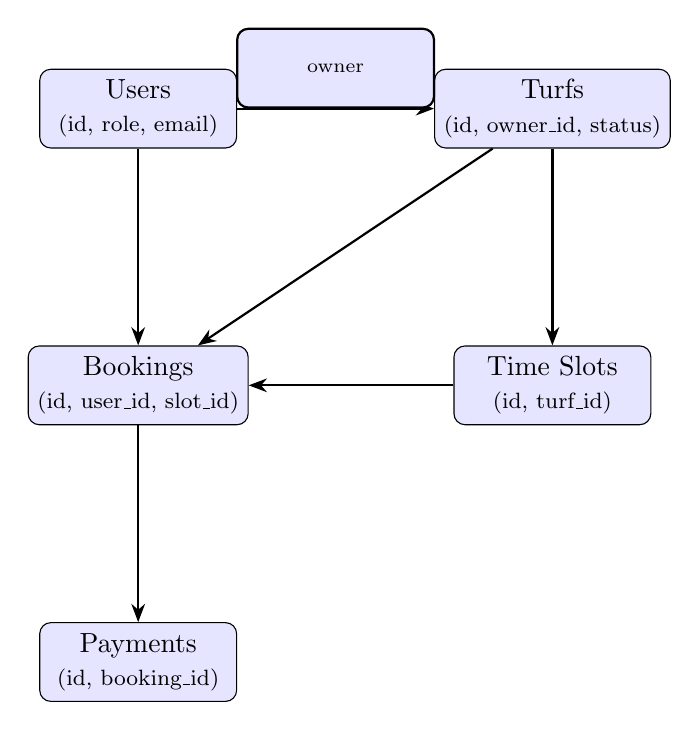
\begin{tikzpicture}[node distance=2.5cm, every node/.style={rectangle, draw, fill=blue!10, rounded corners, minimum width=2.5cm, minimum height=1cm, align=center}]
        \node (users) {Users \\ \footnotesize (id, role, email)};
        \node (turfs) [right=of users] {Turfs \\ \footnotesize (id, owner\_id, status)};
        \node (slots) [below=of turfs] {Time Slots \\ \footnotesize (id, turf\_id)};
        \node (bookings) [below=of users] {Bookings \\ \footnotesize (id, user\_id, slot\_id)};
        \node (payments) [below=of bookings] {Payments \\ \footnotesize (id, booking\_id)};

        \draw [thick, -{Stealth}] (users) -- node[above] {\scriptsize owner} (turfs);
        \draw [thick, -{Stealth}] (users) -- (bookings);
        \draw [thick, -{Stealth}] (turfs) -- (slots);
        \draw [thick, -{Stealth}] (turfs) -- (bookings);
        \draw [thick, -{Stealth}] (slots) -- (bookings);
        \draw [thick, -{Stealth}] (bookings) -- (payments);
    \end{tikzpicture}
    \caption{Relational Database Structure}
    \label{fig:er}
\end{figure}

\newpage
\section{UML Use Case Diagram}
\begin{figure}[h]
    \centering
    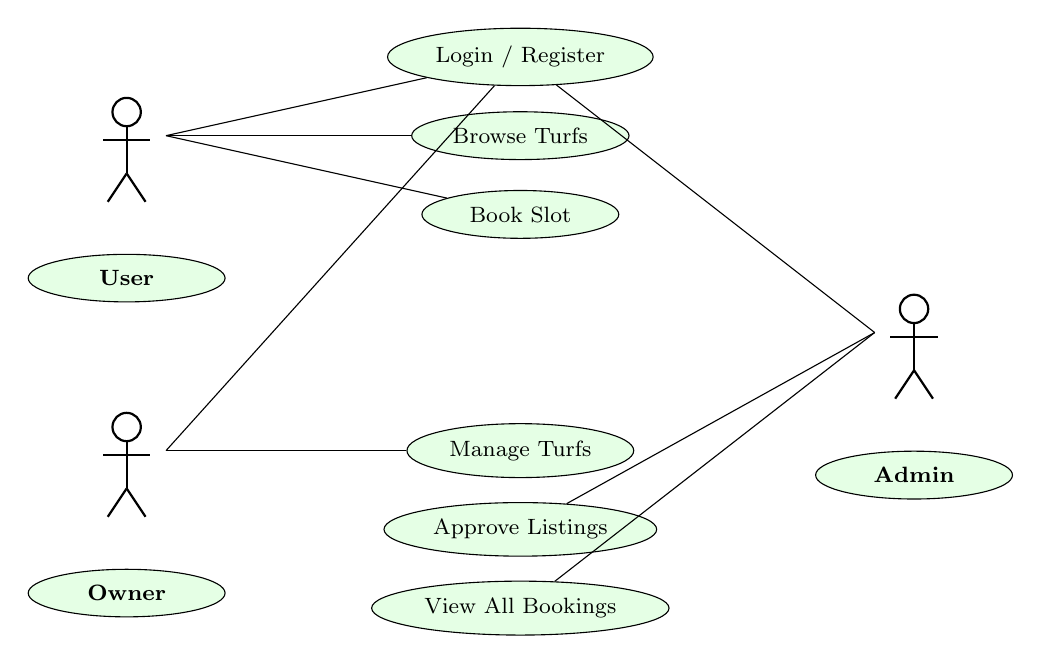
\begin{tikzpicture}[node distance=1.2cm, every node/.style={ellipse, draw, fill=green!10, minimum width=2.5cm, align=center, font=\footnotesize}]
        \node (uc1) at (0, 4) {Login / Register};
        \node (uc2) at (0, 3) {Browse Turfs};
        \node (uc3) at (0, 2) {Book Slot};
        \node (uc4) at (0, -1) {Manage Turfs};
        \node (uc5) at (0, -2) {Approve Listings};
        \node (uc6) at (0, -3) {View All Bookings};

        % User Stick Figure
        \begin{scope}[shift={(-5,3)}, scale=0.6]
            \draw[thick] (0,0.5) circle (0.3); \draw[thick] (0,0.2) -- (0,-0.8); \draw[thick] (-0.5,-0.1) -- (0.5,-0.1); \draw[thick] (0,-0.8) -- (-0.4,-1.4); \draw[thick] (0,-0.8) -- (0.4,-1.4);
            \node[below=1.5cm] {\textbf{User}};
        \end{scope}
        % Owner Stick Figure
        \begin{scope}[shift={(-5,-1)}, scale=0.6]
            \draw[thick] (0,0.5) circle (0.3); \draw[thick] (0,0.2) -- (0,-0.8); \draw[thick] (-0.5,-0.1) -- (0.5,-0.1); \draw[thick] (0,-0.8) -- (-0.4,-1.4); \draw[thick] (0,-0.8) -- (0.4,-1.4);
            \node[below=1.5cm] {\textbf{Owner}};
        \end{scope}
        % Admin Stick Figure
        \begin{scope}[shift={(5,0.5)}, scale=0.6]
            \draw[thick] (0,0.5) circle (0.3); \draw[thick] (0,0.2) -- (0,-0.8); \draw[thick] (-0.5,-0.1) -- (0.5,-0.1); \draw[thick] (0,-0.8) -- (-0.4,-1.4); \draw[thick] (0,-0.8) -- (0.4,-1.4);
            \node[below=1.5cm] {\textbf{Admin}};
        \end{scope}

        \draw (uc1) -- (-4.5, 3); \draw (uc2) -- (-4.5, 3); \draw (uc3) -- (-4.5, 3);
        \draw (uc1) -- (-4.5, -1); \draw (uc4) -- (-4.5, -1);
        \draw (uc1) -- (4.5, 0.5); \draw (uc5) -- (4.5, 0.5); \draw (uc6) -- (4.5, 0.5);
    \end{tikzpicture}
    \caption{UML Use Case Diagram}
\end{figure}

\section{UML Sequence Diagram (AJAX Booking)}
\begin{figure}[h]
    \centering
    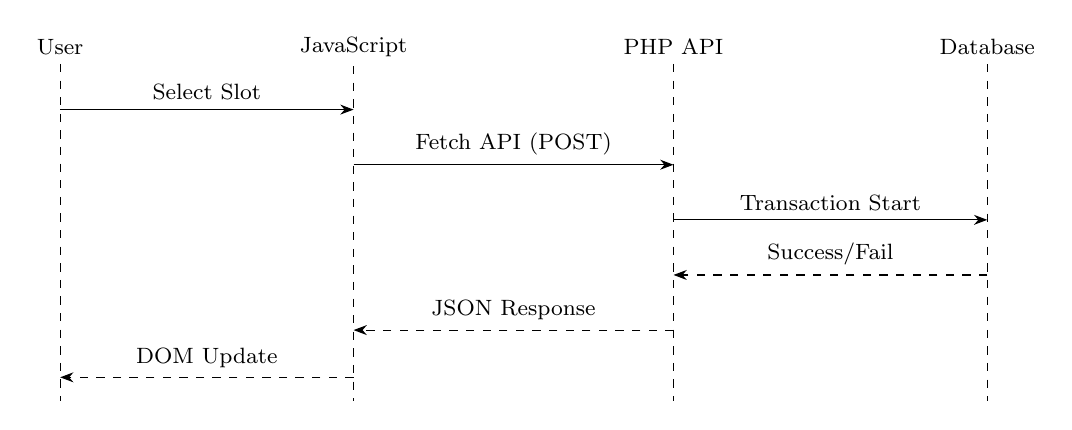
\begin{tikzpicture}[node distance=2.5cm, font=\footnotesize]
        \node (user) {User}; \node (js) [right=of user] {JavaScript}; \node (php) [right=of js] {PHP API}; \node (db) [right=of php] {Database};
        \draw [dashed] (user) -- ++(0,-4.5); \draw [dashed] (js) -- ++(0,-4.5); \draw [dashed] (php) -- ++(0,-4.5); \draw [dashed] (db) -- ++(0,-4.5);

        \draw [-{Stealth}] ($(user)+(0,-0.8)$) -- node[above] {Select Slot} ($(js)+(0,-0.8)$);
        \draw [-{Stealth}] ($(js)+(0,-1.5)$) -- node[above] {Fetch API (POST)} ($(php)+(0,-1.5)$);
        \draw [-{Stealth}] ($(php)+(0,-2.2)$) -- node[above] {Transaction Start} ($(db)+(0,-2.2)$);
        \draw [dashed, -{Stealth}] ($(db)+(0,-2.9)$) -- node[above] {Success/Fail} ($(php)+(0,-2.9)$);
        \draw [dashed, -{Stealth}] ($(php)+(0,-3.6)$) -- node[above] {JSON Response} ($(js)+(0,-3.6)$);
        \draw [dashed, -{Stealth}] ($(js)+(0,-4.2)$) -- node[above] {DOM Update} ($(user)+(0,-4.2)$);
    \end{tikzpicture}
    \caption{Asynchronous Booking Lifecycle}
\end{figure}

% ======================================================
% CHAPTER 4: IMPLEMENTATION
% ======================================================
\chapter{Implementation}
\section{Module Implementation}
\subsection{Authentication \& Role Routing}
The system uses a unified login endpoint. Upon successful password verification via \texttt{password\_verify()}, the server returns the user's role. The frontend JavaScript then routes the user to the appropriate dashboard (User, Owner, or Admin).

\subsection{Concurrency Control}
To prevent two users from booking the same slot at the exact same millisecond, TurfKick uses a two-step verification:
\begin{enumerate}
    \item \textbf{Transaction Isolation}: Using \texttt{SELECT ... FOR UPDATE} to lock the row during the availability check.
    \item \textbf{Unique Constraint}: A MySQL composite unique key on \texttt{(turf\_id, booking\_date, slot\_id)} which acts as a final hardware-level guard.
\end{enumerate}

\section{Code Snippets}
\begin{lstlisting}[language=PHP, caption=Secure Booking Transaction]
$pdo->beginTransaction();
// Lock the check to prevent race conditions
$stmt = $pdo->prepare("SELECT id FROM bookings WHERE turf_id = ? AND booking_date = ? AND slot_id = ? FOR UPDATE");
$stmt->execute([$turf_id, $date, $slot_id]);

if ($stmt->fetch()) {
    $pdo->rollBack(); // Slot was taken during the request
    send_json_response('error', 'Slot already booked.');
}
// Proceed with INSERT...
$pdo->commit();
\end{lstlisting}

\begin{lstlisting}[language=JavaScript, caption=AJAX Availability Check]
async function checkAvailability(turfId, slotId, date) {
    const response = await fetch(`api/check_availability.php?turf_id=${turfId}&slot_id=${slotId}&date=${date}`);
    const result = await response.json();
    if (result.status === 'success' && !result.data.available) {
        updateUI('Slot Booked');
    }
}
\end{lstlisting}

% ======================================================
% CHAPTER 5: TESTING
% ======================================================
\chapter{Testing}
\section{Test Case Scenarios}
\begin{longtable}{|p{1.2cm}|p{3.5cm}|p{4.5cm}|p{3.5cm}|}
\hline
\textbf{ID} & \textbf{Feature} & \textbf{Test Step} & \textbf{Expected Result} \\ \hline
TC01 & Role Access & Login with Admin credentials. & Redirect to Admin Panel. \\ \hline
TC02 & Concurrency & Simultaneous booking of same slot. & One success, one failure. \\ \hline
TC03 & CSRF & Submit booking without token. & Request rejected by API. \\ \hline
TC04 & Sanitization & Input script tag in turf name. & Data escaped correctly. \\ \hline
\end{longtable}

\section{Results}
Testing confirmed that the database locks successfully queued concurrent requests, ensuring no overlapping slots. The AJAX feedback provided users with immediate notification of booking success or failure without page reloads.

% ======================================================
% CHAPTER 6: CONCLUSION
% ======================================================
\chapter{Conclusion}
TurfKick successfully modernizes the turf booking process through a responsive, AJAX-driven architecture. The implementation of robust concurrency controls and role-based access ensures a secure and scalable environment for both users and administrators. Future enhancements will focus on integrating automated SMS notifications and a live payment gateway.

\begin{thebibliography}{9}
\bibitem{php} PHP Manual: PDO Class, \url{https://www.php.net/manual/en/class.pdo.php}
\bibitem{mdn} MDN Web Docs: Fetch API, \url{https://developer.mozilla.org/en-US/docs/Web/API/Fetch_API}
\bibitem{mysql} MySQL 8.0 Reference: Locking, \url{https://dev.mysql.com/doc/refman/8.0/en/innodb-locking-reads.html}
\end{thebibliography}

\end{document}
